\section{Results}
\subsection{What is Porcupine?}
%the general idea 
Porcupine is a graphical workflow editor that automatically produces analysis code from a graphically composed pipeline. By dropping 'nodes' (representing analysis steps) into the workflow editor and by connecting their data inputs and outputs, a pipeline is constructed. Analysis code is then automatically generated from the graphical representation of the pipeline. The code can readily be saved to a script (e.g. a Python, MATLAB, or Docker file) in order to perform the desired analysis. Additionally, the pipeline can be shared or inspected in visual form (PDF/SVG), or saved to a Porcupine specific (.pork) file to continue working on the pipeline at another time.

%the different panels idea
Apart from the visual representation of the pipeline, we provide more functionality to orderly structure one's analysis, as outlined in Fig.~\ref{fig:porcupine-editor}. All functions (the nodes in the graph) that are included in the pipeline are also listed in a separate panel, listing their input parameters, output data, as well as a link to the online documentation of the function. We also provide the option to iterate over any input variable in order to facilitate parallelisation over subjects, sessions, or other variables. All parameters may also be edited in a separate parameter panel of the user interface. This functions as a central storage for important parameters, for example the ones that should be reported in a methods section. Porcupine combines the graphical overview and the parameters to automatically create the analysis code shown in the code window. 
\begin{figure}[!ht]
	\centering
	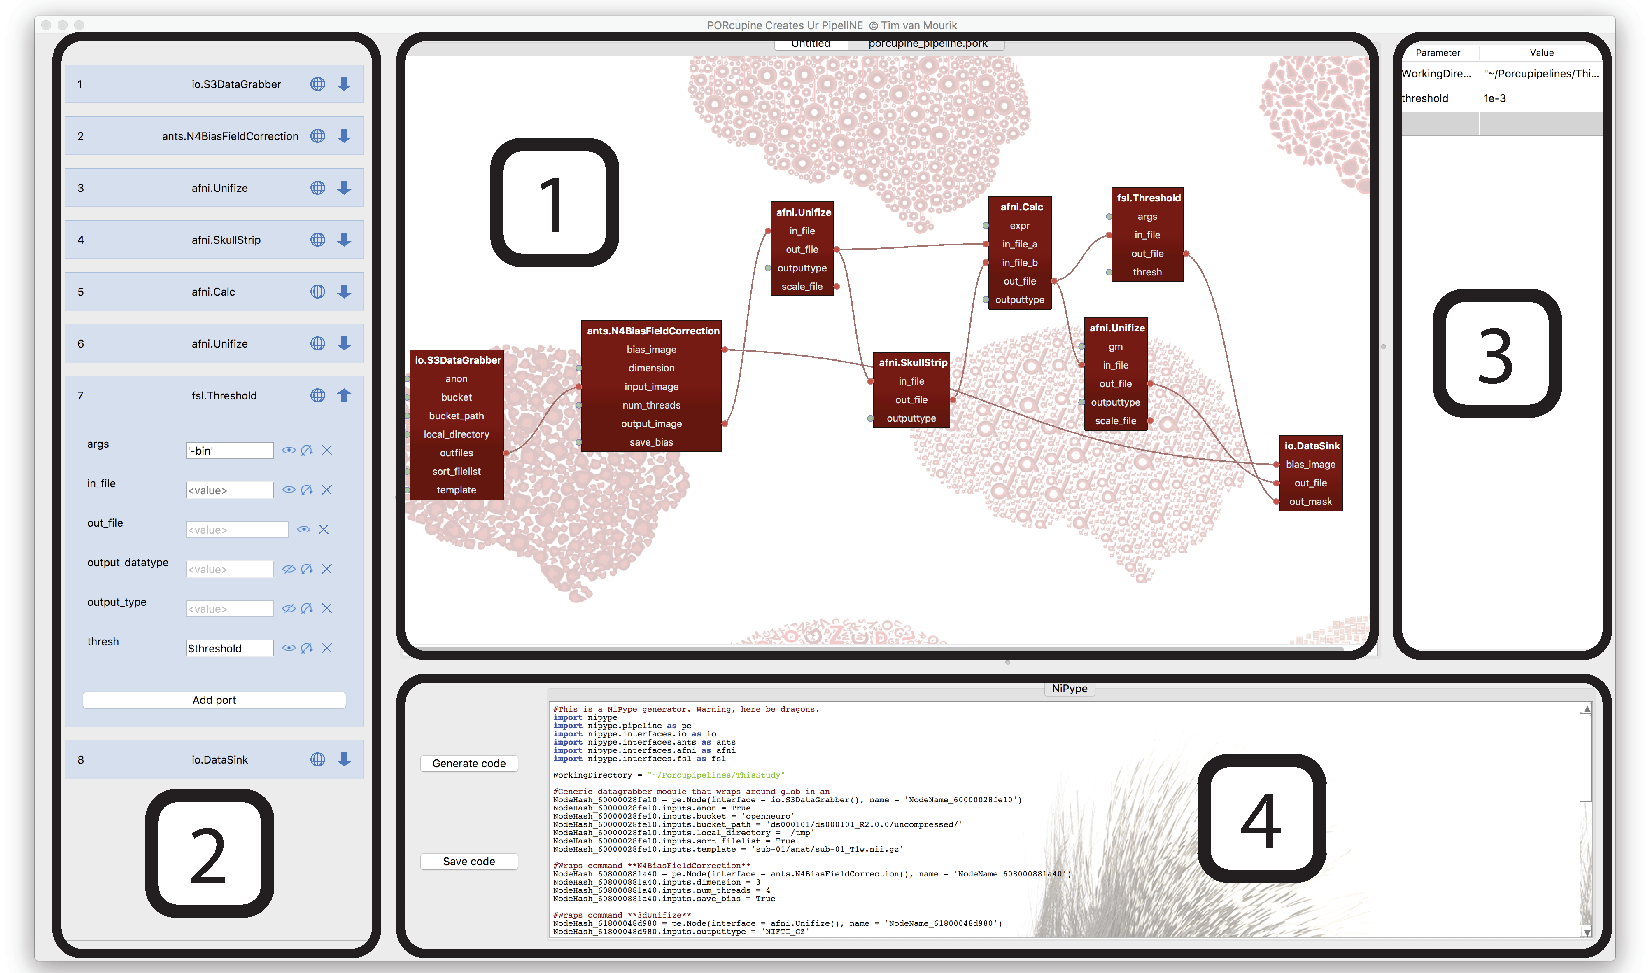
\includegraphics[width=0.9\textwidth, clip=true]{./Chapters/05_Porcupine/./Images/gui_showcase.pdf}
	\caption{A screenshot of a Porcupine workflow. The editor is divided into four panels, each of them targeted at facilitating a more understandable and reproducible analysis. The \emph{workflow editor} (1) provides a visual overview of one's analysis. The functions are all listed in the \emph{node editor} (2), where the parameters for all functions can be orderly stored. This may include links to important parameters that are listed in the \emph{parameter editor} (3), such that an overview of the main analysis settings can be easily viewed and modified. Readily executable analysis code is generated in the \emph{code window} (4)}
	\label{fig:porcupine-editor}
\end{figure}

%scope of this paper
We here focus on code generation that strictly adheres to the Nipype API \cite{Gorgolewski2011}, a Python-based MRI analysis and pipelining package. Nipype is used for its strong focus on uniformity in accessing functions, its link to most major MRI analysis tools, and its emphasis on reproducible science. Porcupine's architecture, however, is in principle agnostic with respect to the specific implementation of the underlying pipelining software. Any package with a consistent interface in the field of e.g. neuroimaging, bioengineering, or astronomy could benefit from using Porcupine's architecture.

%show by example
We first show that we can easily generate a standard fMRI analysis pipeline. After visually dragging and dropping modules, code is automatically created that is usually scripted manually instead. We then show how we facilitate loading data from an online repository, generate a readily executable fMRI pipeline, but also generate a shareable and reproducible analysis environment (using Docker), all with minimal additional effort. This allows for easily scalable analyses that \change{could}{can} be performed locally, but also on computational clusters or with cloud computing, without manual installation of different software packages. 

\subsection{Usage example}
We here show a simple example that constructs a pipeline for a single operation. In three steps, data is loaded, (minimally) processed, and the output is written to disk, as shown in Fig.~\ref{fig:porcupine-simple}. We here show an example that links to an OpenNeuro fMRI data set, but we could load any online data set that is set up according to the BIDS format \cite{Gorgolewski2016}. OpenNeuro's data sets are stored as Amazon repositories (`S3 buckets') and can be loaded by dragging the appropriate module into the workflow editor and typing the name of the bucket into the node editor. Its output can subsequently be connected to a Nipype function node, for example FSL's Brain Extraction Tool. All parameters of the function are listed and can be set in two different ways: either by dragging a link from a previous node's output port to an input port in the next node, or by typing in the parameter in the node editor. Subsequently, output can be written to disk by connecting the desired output to a Nipype DataSink node that collects and stores the data. By pressing the `Generate code` button, the code for this pipeline is automatically generated and can immediately be saved and executed in a Python shell.
\begin{figure}[!ht]
	\centering
	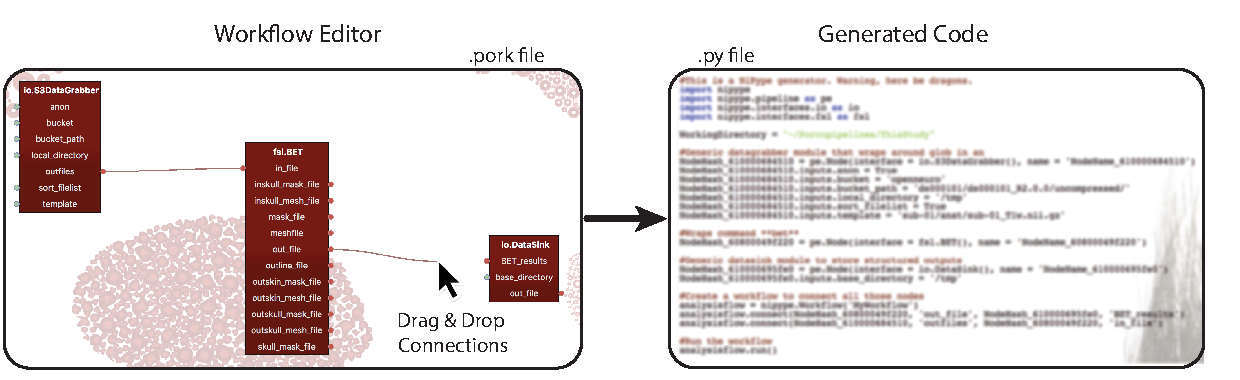
\includegraphics[width=0.9\textwidth, clip=true]{./Chapters/05_Porcupine/./Images/pork_py.pdf}
	\caption{An example of simple workflow. In three steps, this pipeline loads data, processes it, and writes it to disk. This is achieved by connecting the input and output fields from subsequent nodes in the pipeline. The constructed workflow is then transformed in readily executable (Nipype) analysis code.}
	\label{fig:porcupine-simple}
\end{figure}


\subsection{Pipeline sharing}
From a simple example that reads and writes the data, a more complicated pipeline is readily set up. More functionality, i.e. nodes, can be dragged in and connected to quickly build a custom pipeline. As it is commonplace to repeat a single analysis or function for several subjects, sessions, or other variables, every field can be flagged as an `iterator' field. This facilitates looping over variables. Once the pipeline is set up and the code is generated, Nipype offers functionality to construct a visual pipeline graph from custom python code. In Porcupine's proposed use-case, this end point of a standard Nipype pipeline represents the starting point, as shown in Fig.~\ref{fig:porcupine-advanced}. This allows the user to focus on the desired pipeline graph first, and then progress to the manual editing of the generated code.
\begin{figure}[!ht]
	\centering
	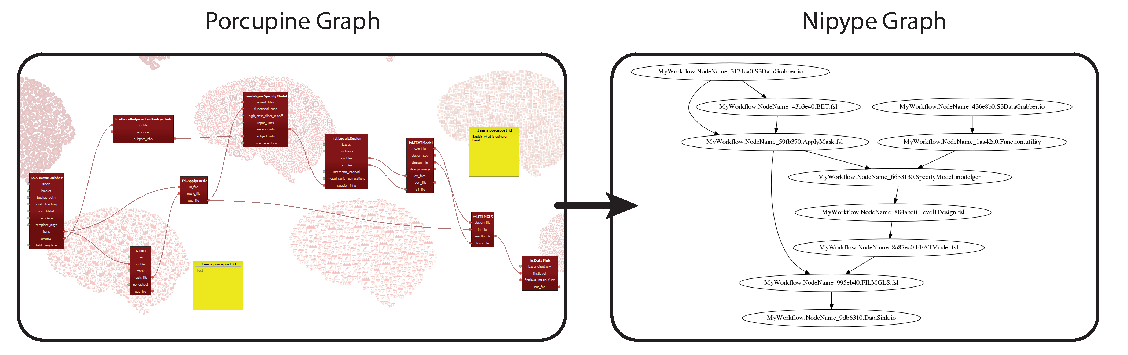
\includegraphics[width=0.9\textwidth, clip=true]{./Chapters/05_Porcupine/./Images/pork_graph.pdf}
	\caption{An example of a more complicated and realistic fMRI preprocessing pipeline. Once the code is generated, this can in turn be transformed into a Nipype graph visualisation. Whereas this is usually the end point for a pipeline in Nipype, we here propose to use a visualisation as a starting point of one's analysis.}
	\label{fig:porcupine-advanced}
\end{figure}

Not only does Porcupine provide a way of setting up a preprocessing  or analysis pipeline, we also provide a means for executing these pipelines in a reproducible environment. In addition to the Python analysis file that is generated, we create a scaffold for a Docker file. Docker (\url{https://www.docker.com}) is an open platform to easily build, run and share applications. The generated Docker file describes a minimal operating system that is required to run the analysis, based on the dependencies of the modules used in the workflow editor. With this Docker file, an image of the full analysis can be built, shared and executed. This provides a simple platform to reproduce results of one's analysis, on the same data set, or on another with only a single change in the data source module. Alternatively, one can use it as a template environment for a new follow-up analysis. As with all generated code, the Docker code is fully customisable to a researcher's need, but our suggested scaffold requires only a single manual edit to be built as a Docker image (see~\nameref{app:docker}). The Docker command will execute the pipeline: load the data from an online repository, process the data, and store only the output data to a local directory. The Docker image includes both the pipeline code and the run environment, and can be shared alongside a paper via DockerHub. The above examples (and many more) as well as extensive documentation and tutorials can be found \href{https://timvanmourik.github.io/Porcupine}{here}.

\subsection{Limitations}
Some features in Nipype have not been implemented. Notably, the JoinNode functionality is not yet accessible from the Porcupine user interface, in which the results from an upstream iterator are aggregated to a single output. Furthermore, custom extensions of Nipype functions are not automatically supported, but we do provide a script to add one's own custom module to Porcupine that would make this functionality accessible. A GUI for this is still an intended point of improvement. In general, feature requests are maintained as \add{\emph{issues} and} \emph{projects} in the \href{https://github.com/TimVanMourik/Porcupine/projects}{GitHub repository}. We encourage people to contribute new ideas or implementations for functionality in terms of modules, new toolboxes, and, most importantly, custom pipelines that can be added to the repository. Details \change{for contributing}{on how to contribute} can be found on the website.

While Porcupine in principle supports all workflow operations, a specific pipeline may well require modules that are not provided within Nipype. It is advised that the user either packages custom code for this into a new module, or manually adds it to the produced code. \change[Reviewer 2]{Porcupine itself functions only as the front-end to the Nipype back-end, but}{We furthermore stress that Porcupine is intended to function as a front-end encapsulation of NiPype, and does not implement the parsing of python files that contain pre-defined nipype pipelines. It also} does not perform type-matching on the input and output of a connection, nor does it perform syntax checking of the manually edited parameters.